\section{分子}\label{sec:1-4}

我们已经学习了氧气的性质,了解到氧气能跟许多物质发生化学反应。为什么物质能够发生这些化学变化呢?
为了深入地研究物质发生化学变化的原因,就要学习有关物质结构的知识。在初中化学里,学习的仅是物质结构的初步知识。

\subsection{分子}

我们经常遇到这样一些问题。例如,在农田用氨水施肥时,为什么远处就能闻到刺激性的氨味?
为什么湿的衣服晒一定时间就干了?为什么蔗糖放进水里,很快就不见了,而水却有了甜味?
这些问题都跟物质的结构有密切的关系。

人们经过长期的科学实验和分析,证明物质都是由许许多多肉眼直接看不见的微粒构成的。
构成物质的微粒有多种,分子是构成物质的一种微粒。
水就是由大量的水分子聚集而成的,一滴水里大约就有十五万亿亿个水分子。
分子很小,如果拿水分子的大小跟乒乓球相比,就好象拿乒乓球的大小跟地球相比一样。
分子这么小,我们单用肉眼是看不到的。现在,人们用电子显微镜把分子放大几十万倍,可以拍摄出分子的照片。
病毒照片(图 \ref{fig:1-10}) 中的每一个小亮点表示一个核蛋白分子,这有力地证明了分子是真实存在的。

\begin{figure}[htbp]
    \centering
    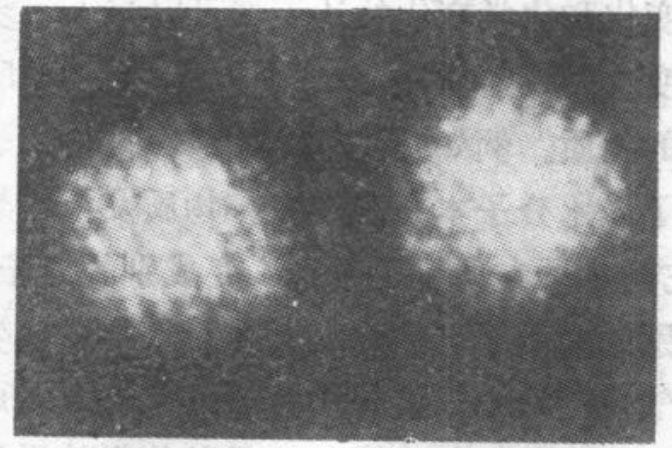
\includegraphics[width=9cm]{../pic/czhx1-ch1-10}
    \caption{用电子显微镜拍摄的由核蛋白分子组成的病毒照片(放大 $20$ 万倍)}\label{fig:1-10}
\end{figure}

分子的质量是非常小的。例如,水分子的质量大约是 $0.000 \; 000 \; 000 \; 000 \; 000 \; 000 \; 000 \; 000 \; 03$ 千克。

分子并不是静止地存在的,而总是在不断地运动着。
远处能闻到刺激性的氨味,湿衣服晒一定时间就干了,正是由于氨分子、水分子不断运动而扩散到空气里去了的缘故。
蔗糖放进水里不见了,也是由于糖分子扩散到水里去了的缘故。

分子间有一定的间隔,一般物体有热胀冷缩的现象,就是由于物质分子间的间隔受热增大,遇冷减小的结果。
这种间隔如果很大,物质就呈气态;如果较小,就呈液态或固态。
所以,一般物质在不同的条件下有三态的变化,主要是由于它们的分子之间的间隔大小发生变化等缘故。

我们学习了分子的知识,对由分子构成的物质发生物理变化和化学变化的认识就可以深入一步。
当发生物理变化的时候,物质的分子本身没有变,所以仍然是原来的物质。
例如,水变成水蒸气,只是分子间的间隔增大了,水分子本身没有变。
物质发生化学变化的时候,它的分子本身起了变化,变成别的分子,所以也就变成别的物质了。
例如,硫在氧气里燃烧变成了二氧化硫气体,是由于硫分子跟氧分子反应变成了二氧化硫分子的缘故。
新生成的分子的化学性质和原来的分子不同。由此可见,
\zhongdian{分子是保持物质化学性质的一种微粒。}

同种物质的分子,性质相同;不同种物质的分子,性质不相同。


\subsection{混和物和纯净物}

\zhongdian{混和物}是由多种成分组成的物质,但是这些成分只是简单地混和在一起,相互间并没有发生化学反应。
例如,空气是氧气、氮气、惰性气体、二氧化碳等多种成分组成的混和物,各种成分间没有发生化学反应。
蔗糖与面粉搀和后,也是一种混和物。混和物里各成分都保持原来的性质。

\zhongdian{纯净物}跟混和物不同,它是由一种物质组成的。
例如,我们学过的氧气,制取氧气所用的氯酸钾,都是纯净物。

分子的知识可以帮助我们比较深入地理解混和物和纯净物的概念。
由分子构成的物质,如果是由不同种分子构成的就是混和物,由同种分子构成的就是纯净物。
例如,空气是由许多氧气分子、氮气分子等不同种分子构成的,所以是混和物。
氧气只是由许多氧气分子构成的,所以是纯净物。

我们研究任何一种物质的性质,都必须取用纯净物。
因为一种物质里如果含有杂质,就会影响这种物质固有的某些性质。

实际上,完全纯净的物质是没有的,通常所谓的纯净物都不是绝对纯净的。
纯净物指的是含杂质很少的具有一定纯度的物质。
凡含杂质的量不至于在生产或科学研究过程中发生有害影响的物质,就可以叫做纯净物。
例如,作半导体材料用的硅,就是从含硅的矿物里提取的。
经提纯,硅的纯度可达 $99.999999999\%$,这种硅叫做高纯硅。
为了适应工农业生产和科学实验的需要,可以用物理或化学的方法,使不纯物质变为比较纯的物质。


\begin{xiti}

\xiaoti{试用分子的知识解释下列现象:}
\begin{xiaoxiaotis}

    \xxt{农用氨水要用密闭的桶、罐、坛或橡皮袋等盛装,以便贮存和运输。}

    \xxt{把湿衣服晾在太阳晒着的地方比晾在没有晒着的地方容易干。}

    \xxt{把蔗糖放在水里,蔗糖就逐渐溶解而看不见了。}

    \xxt{气体受压, 体积缩小。}

\end{xiaoxiaotis}


\xiaoti{下列关于分子的叙述,哪一个是错误的?把错误的叙述加以改正。}
\begin{xiaoxiaotis}

    \xxt{分子是在不断地运动着。}

    \xxt{由分子构成的物质发生物理变化时,分子本身不发生变化,分子间距离也不发生变化。}

    \xxt{由分子构成的物质发生化学变化时,分子本身发生了变化。}

\end{xiaoxiaotis}


\xiaoti{指出下列物质里,哪些属于混和物, 哪些属于纯净物?}
\begin{xiaoxiaotis}

    \xxt{氧化镁,} \xxt{空气,}  \xxt{氧气,} \xxt{液态氧,}  \xxt{铁粉,}

    \xxt{二氧化碳,} \xxt{氯酸钾跟二氧化锰混和并加热制取氧气后的剩余物。}

\end{xiaoxiaotis}

\end{xiti}

